\documentclass{standalone}
\usepackage{tikz}
\usetikzlibrary{patterns, positioning}

\begin{document}
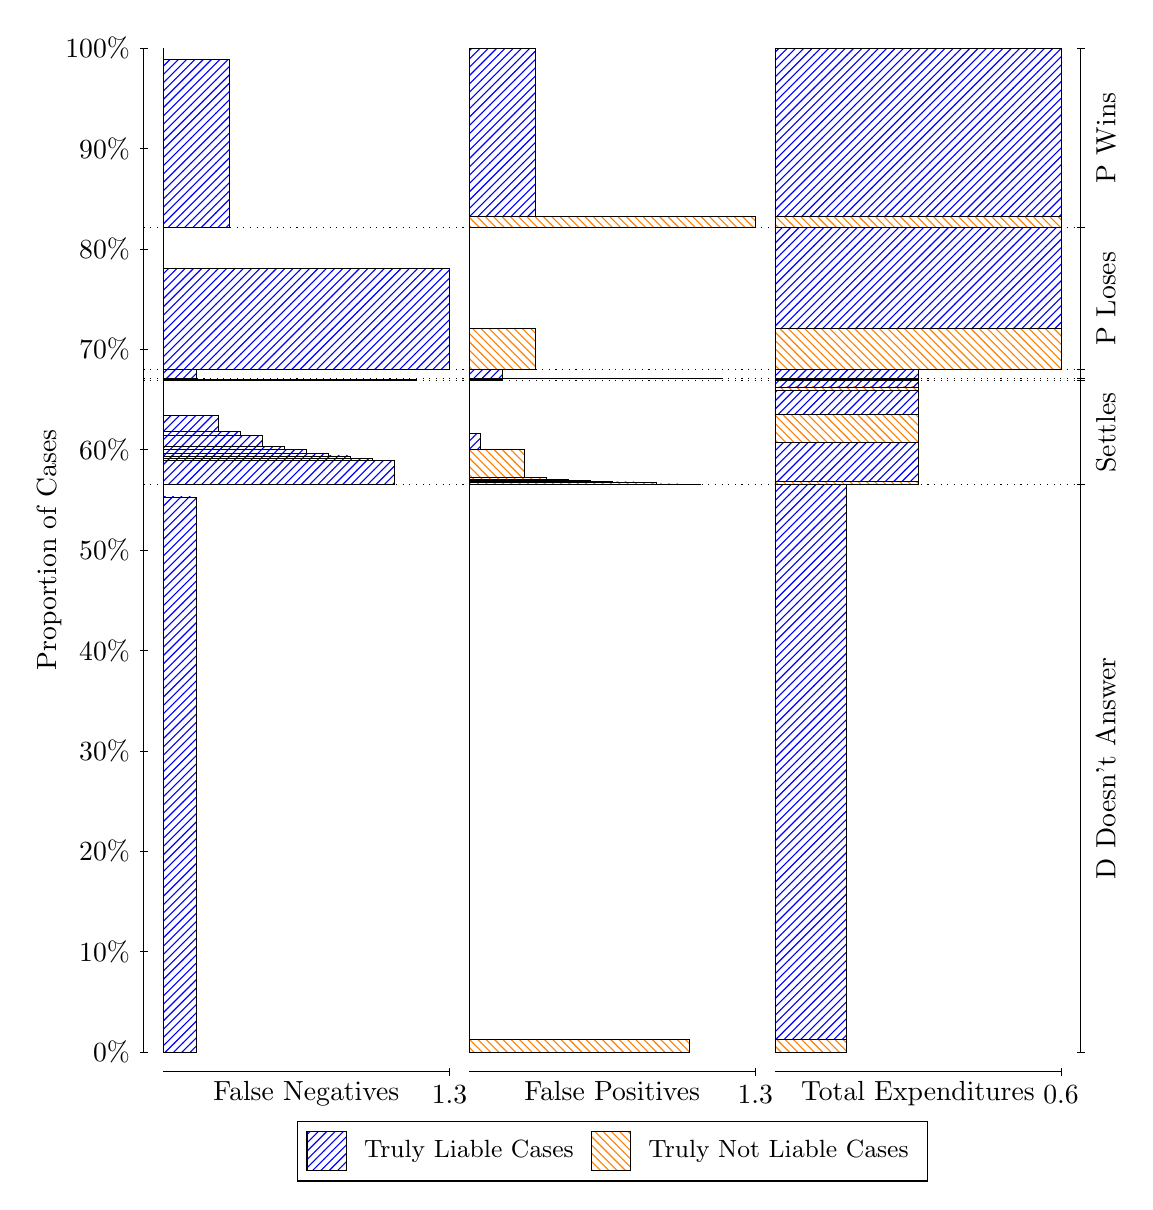
\begin{tikzpicture}
\draw[black, very thin] (1.5,1.75) -- (1.5,14.5);
\node[rotate=90, anchor=center] at (0.3, 8.125) {Proportion of Cases};
\draw[black, very thin] (1.45,1.75) -- (1.55,1.75);
\node[anchor=east] at (1.45, 1.75) {0\%};
\draw[black, very thin] (1.45,3.025) -- (1.55,3.025);
\node[anchor=east] at (1.45, 3.025) {10\%};
\draw[black, very thin] (1.45,4.3) -- (1.55,4.3);
\node[anchor=east] at (1.45, 4.3) {20\%};
\draw[black, very thin] (1.45,5.575) -- (1.55,5.575);
\node[anchor=east] at (1.45, 5.575) {30\%};
\draw[black, very thin] (1.45,6.85) -- (1.55,6.85);
\node[anchor=east] at (1.45, 6.85) {40\%};
\draw[black, very thin] (1.45,8.125) -- (1.55,8.125);
\node[anchor=east] at (1.45, 8.125) {50\%};
\draw[black, very thin] (1.45,9.4) -- (1.55,9.4);
\node[anchor=east] at (1.45, 9.4) {60\%};
\draw[black, very thin] (1.45,10.675) -- (1.55,10.675);
\node[anchor=east] at (1.45, 10.675) {70\%};
\draw[black, very thin] (1.45,11.95) -- (1.55,11.95);
\node[anchor=east] at (1.45, 11.95) {80\%};
\draw[black, very thin] (1.45,13.225) -- (1.55,13.225);
\node[anchor=east] at (1.45, 13.225) {90\%};
\draw[black, very thin] (1.45,14.5) -- (1.55,14.5);
\node[anchor=east] at (1.45, 14.5) {100\%};

\draw[black, very thin] (13.4,1.75) -- (13.4,14.5);
\draw[black, very thin] (13.35,1.75) -- (13.45,1.75);
\node[anchor=west] at (13.35, 1.75) {};
\draw[black, very thin] (13.35,8.9579) -- (13.45,8.9579);
\node[anchor=west] at (13.35, 8.9579) {};
\draw[black, very thin] (13.35,10.28) -- (13.45,10.28);
\node[anchor=west] at (13.35, 10.28) {};
\draw[black, very thin] (13.35,10.305) -- (13.45,10.305);
\node[anchor=west] at (13.35, 10.305) {};
\draw[black, very thin] (13.35,10.419) -- (13.45,10.419);
\node[anchor=west] at (13.35, 10.419) {};
\draw[black, very thin] (13.35,12.219) -- (13.45,12.219);
\node[anchor=west] at (13.35, 12.219) {};
\draw[black, very thin] (13.35,14.5) -- (13.45,14.5);
\node[anchor=west] at (13.35, 14.5) {};

\draw[black, very thin, pattern color=blue, pattern=north east lines] (1.75,1.75) rectangle (2.1692,8.8004);
\draw[black, very thin, pattern color=orange, pattern=north west lines] (1.75,8.8004) rectangle (1.75,8.9579);
\draw[black, very thin, pattern color=blue, pattern=north east lines] (1.75,8.9579) rectangle (4.6846,9.26);
\draw[black, very thin, pattern color=blue, pattern=north east lines] (1.75,9.26) rectangle (4.4051,9.2912);
\draw[black, very thin, pattern color=blue, pattern=north east lines] (1.75,9.2912) rectangle (4.1256,9.3204);
\draw[black, very thin, pattern color=blue, pattern=north east lines] (1.75,9.3204) rectangle (3.8462,9.3509);
\draw[black, very thin, pattern color=blue, pattern=north east lines] (1.75,9.3509) rectangle (3.5667,9.3985);
\draw[black, very thin, pattern color=blue, pattern=north east lines] (1.75,9.3985) rectangle (3.2872,9.4454);
\draw[black, very thin, pattern color=blue, pattern=north east lines] (1.75,9.4454) rectangle (3.0077,9.5796);
\draw[black, very thin, pattern color=blue, pattern=north east lines] (1.75,9.5796) rectangle (2.7282,9.6269);
\draw[black, very thin, pattern color=blue, pattern=north east lines] (1.75,9.6269) rectangle (2.4487,9.8369);
\draw[black, very thin, pattern color=orange, pattern=north west lines] (1.75,9.8369) rectangle (1.75,10.28);
\draw[black, very thin, pattern color=blue, pattern=north east lines] (1.75,10.28) rectangle (4.9641,10.291);
\draw[black, very thin, pattern color=orange, pattern=north west lines] (1.75,10.291) rectangle (1.75,10.305);
\draw[black, very thin, pattern color=blue, pattern=north east lines] (1.75,10.305) rectangle (2.1692,10.416);
\draw[black, very thin, pattern color=orange, pattern=north west lines] (1.75,10.416) rectangle (1.75,10.419);
\draw[black, very thin, pattern color=blue, pattern=north east lines] (1.75,10.419) rectangle (5.3833,11.702);
\draw[black, very thin, pattern color=orange, pattern=north west lines] (1.75,11.702) rectangle (1.75,12.219);
\draw[black, very thin, pattern color=blue, pattern=north east lines] (1.75,12.219) rectangle (2.5885,14.359);
\draw[black, very thin, pattern color=orange, pattern=north west lines] (1.75,14.359) rectangle (1.75,14.5);
\draw[black, very thin, pattern color=orange, pattern=north west lines] (5.6333,1.75) rectangle (8.4282,1.9076);
\draw[black, very thin, pattern color=blue, pattern=north east lines] (5.6333,1.9076) rectangle (5.6333,8.9579);
\draw[black, very thin, pattern color=orange, pattern=north west lines] (5.6333,8.9579) rectangle (8.5679,8.9624);
\draw[black, very thin, pattern color=orange, pattern=north west lines] (5.6333,8.9624) rectangle (8.2885,8.965);
\draw[black, very thin, pattern color=orange, pattern=north west lines] (5.6333,8.965) rectangle (8.009,8.9813);
\draw[black, very thin, pattern color=orange, pattern=north west lines] (5.6333,8.9813) rectangle (7.7295,8.9887);
\draw[black, very thin, pattern color=orange, pattern=north west lines] (5.6333,8.9887) rectangle (7.45,8.9975);
\draw[black, very thin, pattern color=orange, pattern=north west lines] (5.6333,8.9975) rectangle (7.1705,8.9995);
\draw[black, very thin, pattern color=orange, pattern=north west lines] (5.6333,8.9995) rectangle (7.1705,9.0109);
\draw[black, very thin, pattern color=orange, pattern=north west lines] (5.6333,9.0109) rectangle (6.891,9.0238);
\draw[black, very thin, pattern color=orange, pattern=north west lines] (5.6333,9.0238) rectangle (6.6115,9.0477);
\draw[black, very thin, pattern color=orange, pattern=north west lines] (5.6333,9.0477) rectangle (6.3321,9.4006);
\draw[black, very thin, pattern color=blue, pattern=north east lines] (5.6333,9.4006) rectangle (5.7731,9.6105);
\draw[black, very thin, pattern color=blue, pattern=north east lines] (5.6333,9.6105) rectangle (5.6333,10.28);
\draw[black, very thin, pattern color=orange, pattern=north west lines] (5.6333,10.28) rectangle (6.0526,10.293);
\draw[black, very thin, pattern color=blue, pattern=north east lines] (5.6333,10.293) rectangle (5.6333,10.305);
\draw[black, very thin, pattern color=orange, pattern=north west lines] (5.6333,10.305) rectangle (8.8474,10.308);
\draw[black, very thin, pattern color=blue, pattern=north east lines] (5.6333,10.308) rectangle (6.0526,10.419);
\draw[black, very thin, pattern color=orange, pattern=north west lines] (5.6333,10.419) rectangle (6.4718,10.936);
\draw[black, very thin, pattern color=blue, pattern=north east lines] (5.6333,10.936) rectangle (5.6333,12.219);
\draw[black, very thin, pattern color=orange, pattern=north west lines] (5.6333,12.219) rectangle (9.2667,12.36);
\draw[black, very thin, pattern color=blue, pattern=north east lines] (5.6333,12.36) rectangle (6.4718,14.5);
\draw[black, very thin, pattern color=orange, pattern=north west lines] (9.5167,1.75) rectangle (10.425,1.9076);
\draw[black, very thin, pattern color=blue, pattern=north east lines] (9.5167,1.9076) rectangle (10.425,8.9579);
\draw[black, very thin, pattern color=orange, pattern=north west lines] (9.5167,8.9579) rectangle (11.333,8.9995);
\draw[black, very thin, pattern color=blue, pattern=north east lines] (9.5167,8.9995) rectangle (11.333,9.4938);
\draw[black, very thin, pattern color=orange, pattern=north west lines] (9.5167,9.4938) rectangle (11.333,9.8467);
\draw[black, very thin, pattern color=blue, pattern=north east lines] (9.5167,9.8467) rectangle (11.333,10.149);
\draw[black, very thin, pattern color=orange, pattern=north west lines] (9.5167,10.149) rectangle (11.333,10.197);
\draw[black, very thin, pattern color=blue, pattern=north east lines] (9.5167,10.197) rectangle (11.333,10.28);
\draw[black, very thin, pattern color=orange, pattern=north west lines] (9.5167,10.28) rectangle (11.333,10.293);
\draw[black, very thin, pattern color=blue, pattern=north east lines] (9.5167,10.293) rectangle (11.333,10.305);
\draw[black, very thin, pattern color=orange, pattern=north west lines] (9.5167,10.305) rectangle (11.333,10.308);
\draw[black, very thin, pattern color=blue, pattern=north east lines] (9.5167,10.308) rectangle (11.333,10.419);
\draw[black, very thin, pattern color=orange, pattern=north west lines] (9.5167,10.419) rectangle (13.15,10.936);
\draw[black, very thin, pattern color=blue, pattern=north east lines] (9.5167,10.936) rectangle (13.15,12.219);
\draw[black, very thin, pattern color=orange, pattern=north west lines] (9.5167,12.219) rectangle (13.15,12.36);
\draw[black, very thin, pattern color=blue, pattern=north east lines] (9.5167,12.36) rectangle (13.15,14.5);
\draw[black, dotted] (1.5,8.9579) -- (13.4,8.9579);
\draw[black, dotted] (1.5,10.28) -- (13.4,10.28);
\draw[black, dotted] (1.5,10.305) -- (13.4,10.305);
\draw[black, dotted] (1.5,10.419) -- (13.4,10.419);
\draw[black, dotted] (1.5,12.219) -- (13.4,12.219);
\draw[black, very thin] (1.75,1.5) -- (5.3833,1.5);
\node[anchor=north] at (3.5667, 1.5) {False Negatives};
\draw[black, very thin] (5.3833,1.45) -- (5.3833,1.55);
\node[anchor=north] at (5.3833, 1.45) {1.3};

\draw[black, very thin] (5.6333,1.5) -- (9.2667,1.5);
\node[anchor=north] at (7.45, 1.5) {False Positives};
\draw[black, very thin] (9.2667,1.45) -- (9.2667,1.55);
\node[anchor=north] at (9.2667, 1.45) {1.3};

\draw[black, very thin] (9.5167,1.5) -- (13.15,1.5);
\node[anchor=north] at (11.333, 1.5) {Total Expenditures};
\draw[black, very thin] (13.15,1.45) -- (13.15,1.55);
\node[anchor=north] at (13.15, 1.45) {0.6};

\node[black, centered, rotate=90] at (13.72, 5.354) {D Doesn't Answer};
\node[black, centered, rotate=90] at (13.72, 9.6187) {Settles};


\node[black, centered, rotate=90] at (13.72, 11.319) {P Loses};
\node[black, centered, rotate=90] at (13.72, 13.359) {P Wins};

\draw (7.449999999999999,1.5) node[draw=none] (baseCoordinate) {};
\begin{scope}[align=center]
        \matrix[scale=0.5, draw=black, below=0.5cm of baseCoordinate, nodes={draw}, column sep=0.1cm]{
            \node[rectangle, draw, minimum width=0.5cm, minimum height=0.5cm, pattern=north east lines, pattern color=blue] {}; &
            \node[draw=none, font=\small] (B) {Truly Liable Cases}; &
            \node[rectangle, draw, minimum width=0.5cm, minimum height=0.5cm, pattern=north west lines, pattern color=orange] {}; &
            \node[draw=none, font=\small] (B) {Truly Not Liable Cases}; \\
            };
\end{scope}

\end{tikzpicture}
\end{document}